\chapter{Results}
\label{sec:results}

\section{Findings from the Simulations}
- Wie in Vorversuchen schon bemerkt: QE-Schema produziert numerische Fehler, die sich darin zeigen, dass Preise mehrfach in der Simulation vorkommen. Bei korrekter Simulation ist der häufigste Preis im ersten Pfad im einstelligen Bereich, bei Fehlern im Hunderter- oder Tausenderbereich.
- Abbildung \ref{fig:max_number_of_same_prices_distribution} zeigt die Verteilung, man sieht einen Peak bei 1, was darauf hindeutet, dass die meisten Simulationen korrekt sind. Man sieht aber auch, dass es einige Simulationen gibt, wo der selbe Preis bis zu 250000 mal vorkommt, hier kam es zu numerischen Fehlern. Bei diesen Simulationen stellt man fest, dass, wenn es das erste Mal zu numerischen Fehlern kommt, der Rest der Zeitreihe den selben Preis hat. Bei Simulationen mit 250000 gleichen Preises kam es also sehr früh in der Zeitreihe zu einem numerischen Fehler.

\begin{figure}
    \centering
    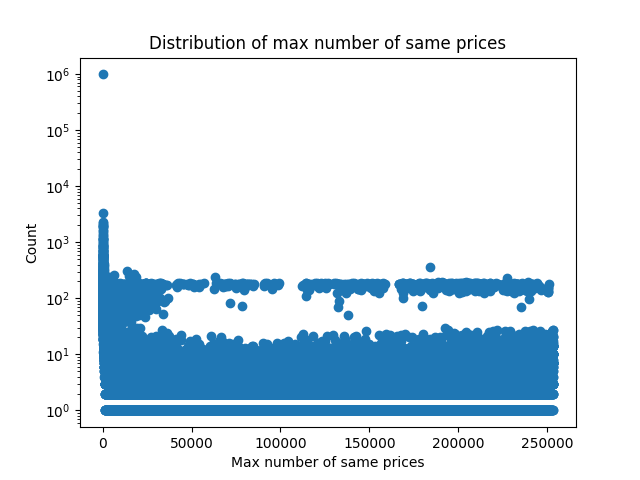
\includegraphics[width=0.8\textwidth]{img/max_number_of_same_prices_distribution.png}
    \caption{Distribution of the maximum number of the same prices in the first path of the simulation}
    \label{fig:max_number_of_same_prices_distribution}
\end{figure}

- Für die weitere Untersuchung sollen solche Simulationen ausgeschlossen werden, da sie nicht korrekt sind. Da es durchaus möglich ist, dass es auch bei korrekter Simulation zu gleichen Preisen kommt, wird ein Schwellwert gesucht, sodass möglichst viele korrekte Simulationen in der Untersuchung bleiben. Abbildung \ref{fig:max_number_of_same_prices_cumulative_percentage} zeigt für verschiedene Schwellwerte (die maximale Anzahl an gleichen Preisen) den kumulativen Anteil der Simulationen, die diesen Schwellwert nicht überschreiten. Wählt man den Schwellwert 1, also nur Simulationen, bei denen nie ein Preis mehrfach vorkommt, verbleiben bleiben 68.40\% der Simulation. Je höher man den Schwellwert setzt, desto weniger Simulationen fallen weg, aber unter Umständen verbleiben auch Simulationen, die numerische Fehler enthalten. Das betrifft aber nur sehr wenige Simulationen, der Anteil an inkludierten Simulationen steigt fast gar nicht. Für die späteren Untersuchungen werden also alle Simulationen entfernt, bei denen der selbe Preis mehr als einmal vorkommt.

\begin{figure}
    \centering
    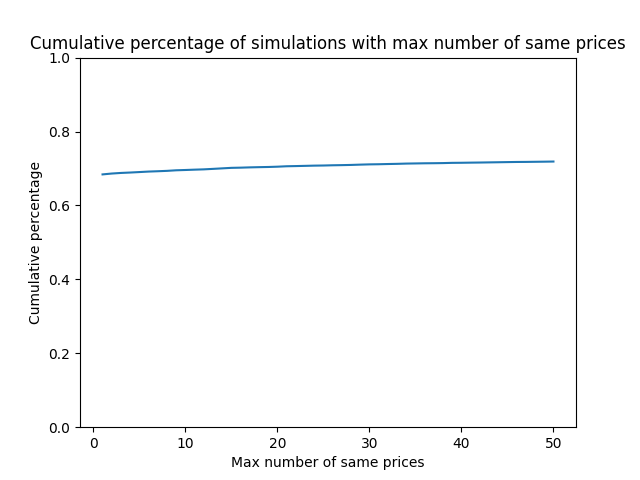
\includegraphics[width=0.8\textwidth]{img/max_number_of_same_prices_cumulative_percentage.png}
    \caption{Cumulative percentage of simulations that do not exceed the maximum number of same prices}
    \label{fig:max_number_of_same_prices_cumulative_percentage}
\end{figure}

\section{Comparing Distributions with the Kolmogorov-Smirnov-Test}

\section{Comparing the Tails of the Distributions}